\chapter{中央データベースとローカルデータベースのデータ同期ツールに関する開発}

開発した機能が生産時に十分であるかどうか見積もりは今後の開発を効率よく進めていく上で重要である。
生産時のデータの数や量を想定してその際のシステム性能を見積もることで、今の実装で十分かどうか、改善が必要な場合どのように改善すればいいかを知ることができる。
中央データベースとローカルデータベースのデータ同期機能に関して処理時間評価を行った。
詳細について以下で説明する。

\section{サーバーの設置場所による処理時間の違い}
4章で述べたように、中央データベースはチェコに設置されている。
そのため試験結果のアップロードに関して、各組み立て機関から接続しデータ送信する処理時間は、機関の場所に大きく依存すると考えられる。
世界的にデータ同期ツールが不自由なく動くことに向けた開発、改善に役立てることを目的として、データを送信する処理時間を、以下の3つの場所に置かれているサーバーを用いて測定した。

\begin{itemize}
  \item 日本、高エネルギー加速器研究所(KEK) 
  \item アメリカ、バークレー研究所(LBL)
  \item スイス、欧州原子核研究機構(CERN)
\end{itemize}

各サーバーの性能を表\ref{server_spec}に示す。また各サーバーが置かれている場所の位置関係を図\ref{server_geometry}に示す。

\begin{table}[tbp]
\caption[サーバーの性能一覧]{サーバーの性能一覧}
\label{server_spec}
\scalebox{0.9}{
  \begin{tabular}{|l|llll|l|l|} \hline
    設置機関 & CPU & & & & Memory & Disk \\
     & Type & Core & Thread & Clock speed[GHz]& [kB] & [GB] \\ \hline 
    KEK & Intel(R) Core(TM) i7-9700K & 8 & 16 & 3.6 & 32,658,772 & 1800 + 1800\\
    LBL & Intel(R) Core(TM) i7-8700 & 6 & 12 & 3.7 & 32,628,000 & 233\\
    CERN & Intel(R) Core(TM) i7-4790 & 4 & 8 & 3.6 & 32,686,404 & 238.5 + 3700 + 3700\\ \hline
  \end{tabular}
}
\end{table}


\begin{figure}[bpt]\centering
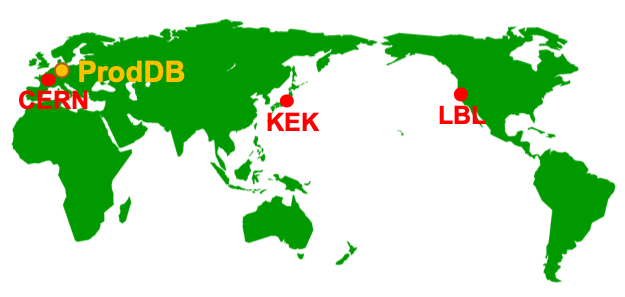
\includegraphics[width=10cm]{server_geometry}
\caption[各サーバの位置関係]{各サーバの位置関係}
\label{server_geometry}
\end{figure}

これらのサーバーは実際に生産の際に使用するものと同程度の性能を持ち、サーバーが置かれている環境も生産時と同じであるとしている。
回線の混雑具合などによる処理時間の低下は、本測定では考慮に入れていない。

\subsection{データ同期ツールに使用するAPI}
中央データベースのデータ取得には、用意されているAPIのサービスを使用している。
ローカルデータベースとのデータ同期ツールの中で主に使用しているAPIを表\ref{pd_API}に示す。

\begin{table}[tbp]
  \begin{center}
  \caption[データ同期ツールの中で使用しているAPI]{データ同期ツールの中で使用したAPI}
  \label{pd_API}
  \scalebox{0.7}{
    \begin{tabular}{|lll|} \hline
      関数名 & 処理の内容 & 本ツールでの使用用途\\ \hline
      getComponent            & 
      登録した装置情報の取得 & 主にダウンロード時におけるモジュールやチップの情報取得に用いる。\\
      uploadTestRunResults    & 
      テスト結果生成 & 読み出し試験結果生成の際に用いる。 \\
      createTestRunAttachment & 
      あるテスト結果に対するバイナリファイルの添付 & 読み出し試験結果生成後にファイルを添付する際に用いる。\\ \hline
    \end{tabular}
  }
  \end{center}
\end{table}

\subsection{API使用にかかる時間}
上述したAPI使用時の処理時間を各サーバーで測定した。
以下の3つの測定を行なった。
\begin{itemize}
  \item getComponentを用いた、登録モジュール情報1つの取得時間測定
  \item createTestRunAttachmentを用いて、ある試験結果ページに1Byteのデータファイルを添付する時間測定
  \item createTestRunAttachmentを用いて、ある試験結果ページに容量の異なるデータファイルを添付、容量に対する時間依存性を測定
\end{itemize}

最初の2項目に関して、各処理時間についてまとめたものを表\ref{getting_1module}、\ref{sendpd_1byte}に示す。
またファイル容量と処理時間の関係を図\ref{datasize_vs_time}に示す。1Byteでの測定点も含んでいる。

\begin{table}[tbp]
  \begin{minipage}[t]{.45\textwidth}
  \begin{center}
  \caption[モジュール情報の取得にかかる時間]{モジュール情報の取得にかかる時間}
  \label{getting_1module}
    \begin{tabular}{|ll|} \hline
      サーバー & 処理時間[秒] \\ \hline
      KEK & 0.49 $\pm$ 0.02 \\ 
      LBL & 0.37 $\pm$ 0.02 \\ 
      CERN & 0.30 $\pm$ 0.04 \\ \hline 
    \end{tabular}
  \end{center}
  \end{minipage}
  \hfill 
  \begin{minipage}[t]{.45\textwidth}
  \begin{center}
  \caption[1Byteのデータファイル添付にかかる処理時間]{1Byteのデータファイル添付にかかる処理時間}
  \label{sendpd_1byte}
    \begin{tabular}{|ll|} \hline
      サーバー & 処理時間[秒] \\ \hline
      KEK & 0.54 $\pm$ 0.04 \\ 
      LBL & 0.34 $\pm$ 0.03 \\ 
      CERN & 0.39 $\pm$ 0.02 \\ \hline 
    \end{tabular}
  \end{center}
  \end{minipage}
\end{table}

\begin{figure}[bpt]\centering
  \begin{center}
    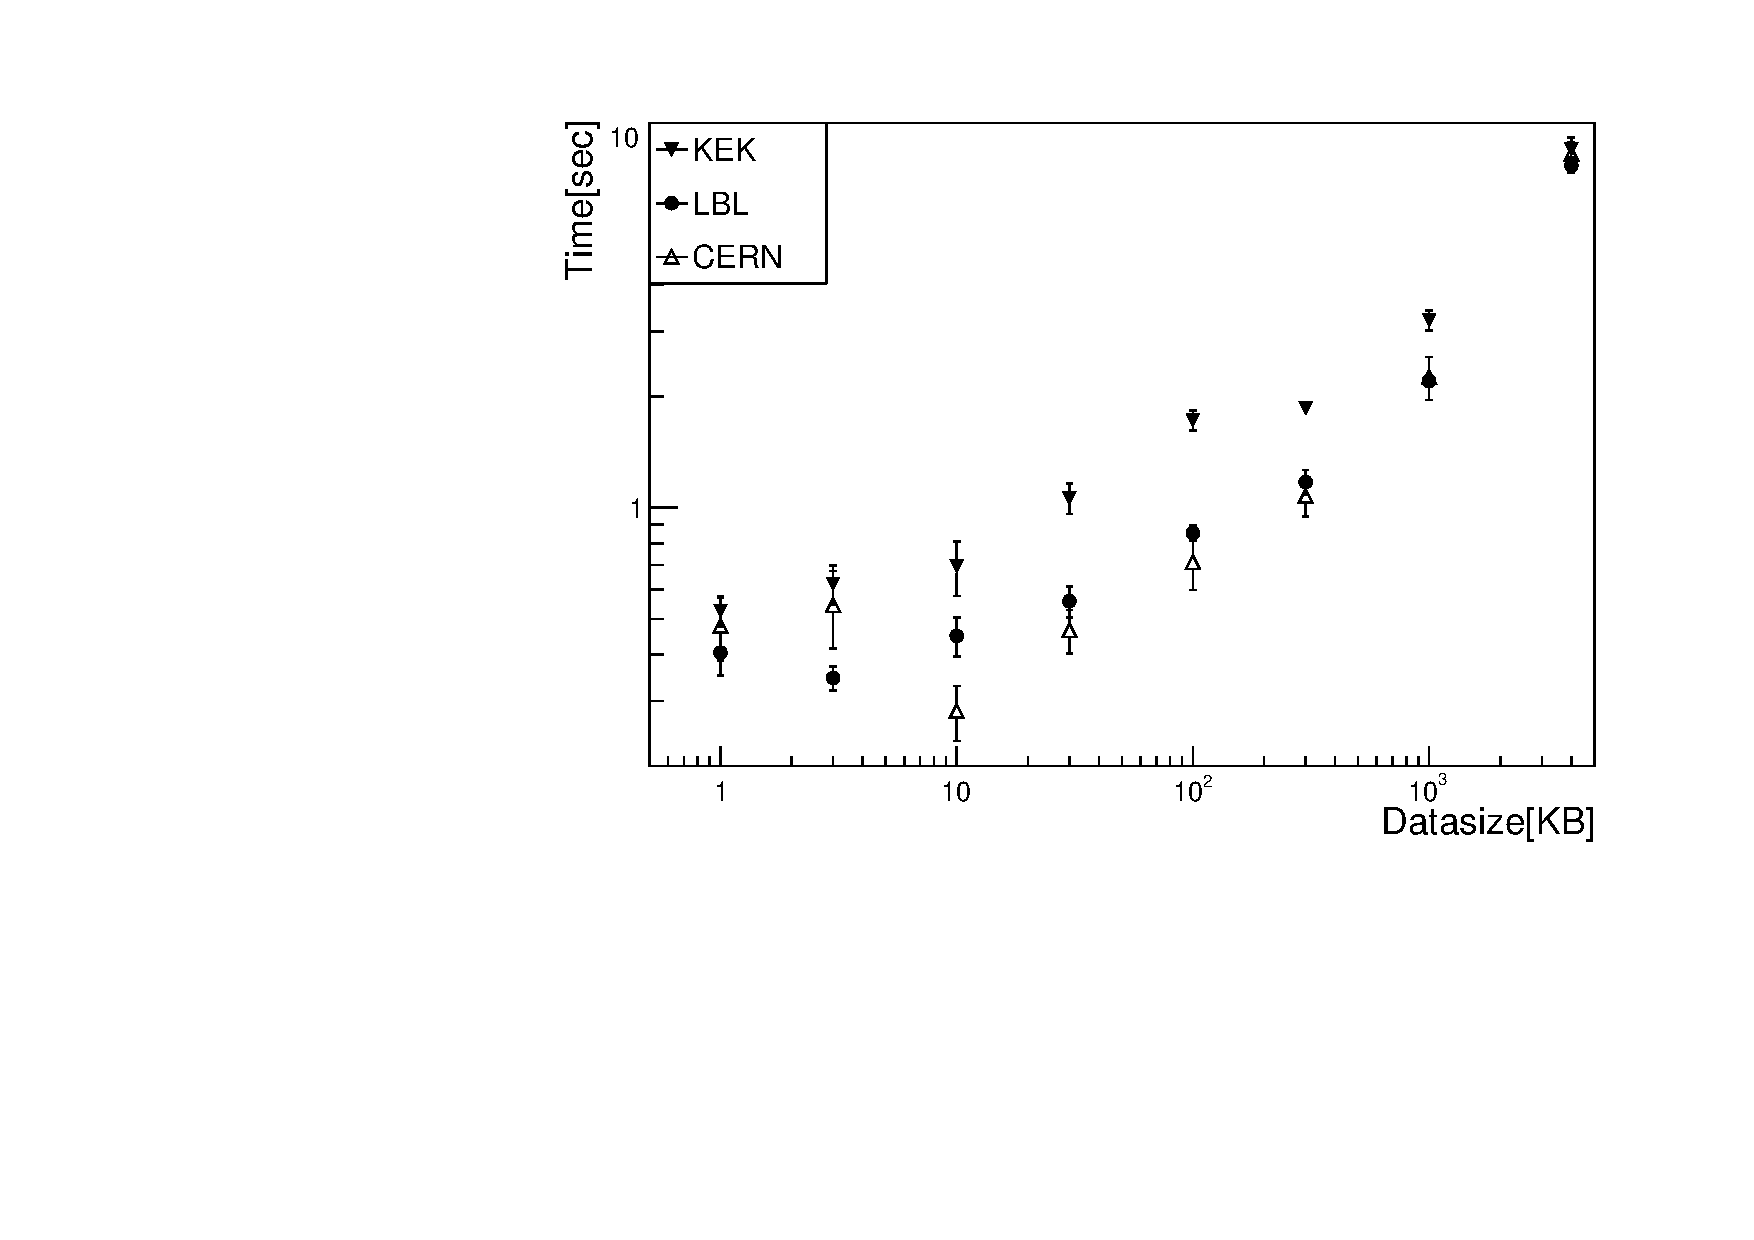
\includegraphics[width=8cm,angle=270]{datasize_vs_time_new.pdf}
  \caption[添付するファイルサイズと処理時間の関係]{添付するファイルサイズと処理時間の関係}
  \label{datasize_vs_time}
  \end{center}

\end{figure}

\section{モジュールIDのダウンロード機能確認と処理時間測定}
\subsection{ダウンロードする情報と構造}
中央データベースから、モジュール及びFEチップの情報をダウンロードする。
それぞれの情報の詳細について以下に示す。
\begin{itemize}
  \item モジュール情報
     \begin{itemize}
       \item シリアルナンバー
       \item FEチップの種類
       \item 登録された機関
       \item FEチップの枚数
     \end{itemize}
  \item FEチップ情報
     \begin{itemize}
       \item シリアルナンバー
       \item FEチップID(モジュール上の位置情報に相当)
       \item 登録された機関
     \end{itemize}
\end{itemize}

ダウンロードされたモジュールのドキュメントの例を以下に示す。
\begin{lstlisting}[caption=モジュール,label=fuga]
{
	"_id" : ObjectId("5fa79114e615fa000a1a5976"),
	"name" : "20UPGR00000001",
	"chipType" : "RD53A",
	"serialNumber" : "20UPGR00000001",
	"chipId" : -1,
	"componentType" : "module",
	"address" : "5fd597fdf7339bbf26b87fb2",
	"children" : 1,
	"sys" : {
		"mts" : ISODate("2020-12-13T04:26:37.989Z"),
		"cts" : ISODate("2020-12-13T04:26:37.989Z"),
		"rev" : 0
	},
	"dbVersion" : 1.01,
	"user_id" : -1,
	"proDB" : true
}
\end{lstlisting}
\begin{lstlisting}[caption=FEチップ,label=fuga]
{
	"_id" : ObjectId("5fa79560e615fa000a1a5a16"),
	"name" : "20UPGFC9999999",
	"chipType" : "RD53A",
	"serialNumber" : "20UPGFC9999999",
	"chipId" : 0,
	"componentType" : "front-end_chip",
	"address" : "5fd597fdf7339bbf26b87fb2",
	"children" : -1,
	"sys" : {
		"mts" : ISODate("2020-12-13T04:26:37.984Z"),
		"cts" : ISODate("2020-12-13T04:26:37.984Z"),
		"rev" : 0
	},
	"dbVersion" : 1.01,
	"user_id" : -1,
	"proDB" : true
}
\end{lstlisting}

\subsection{処理の流れ}

ダウンロード機能における処理の流れのイメージを図\ref{download_algorithm}に示す。

\begin{figure}[bpt]\centering
  \begin{center}
  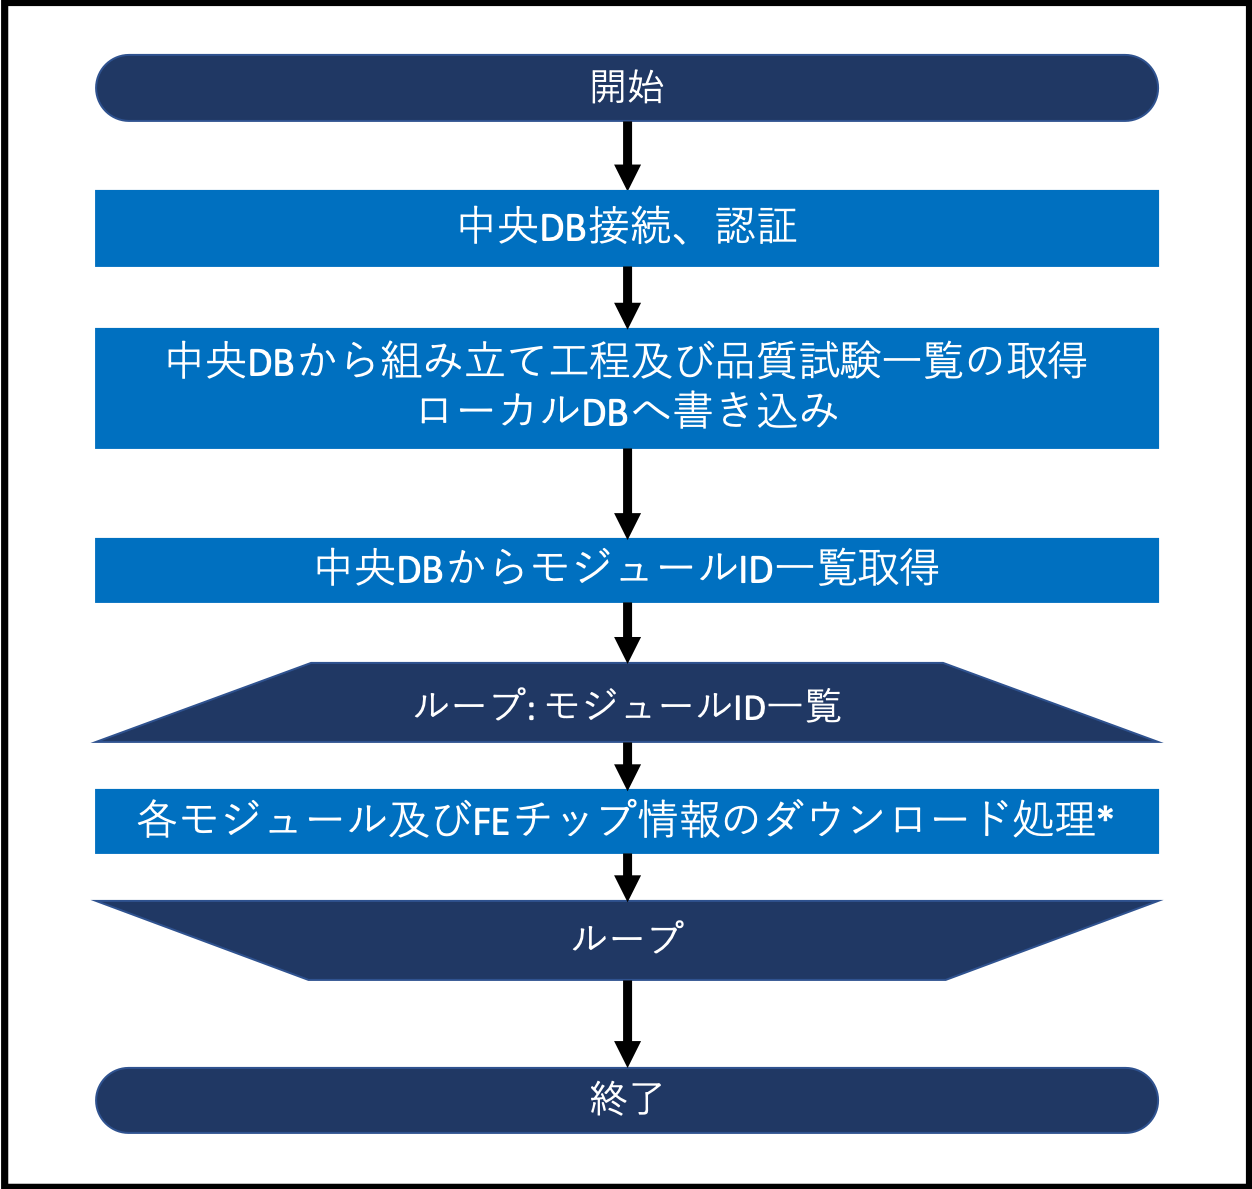
\includegraphics[width=11cm]{download_tool_flow_whole.png}
  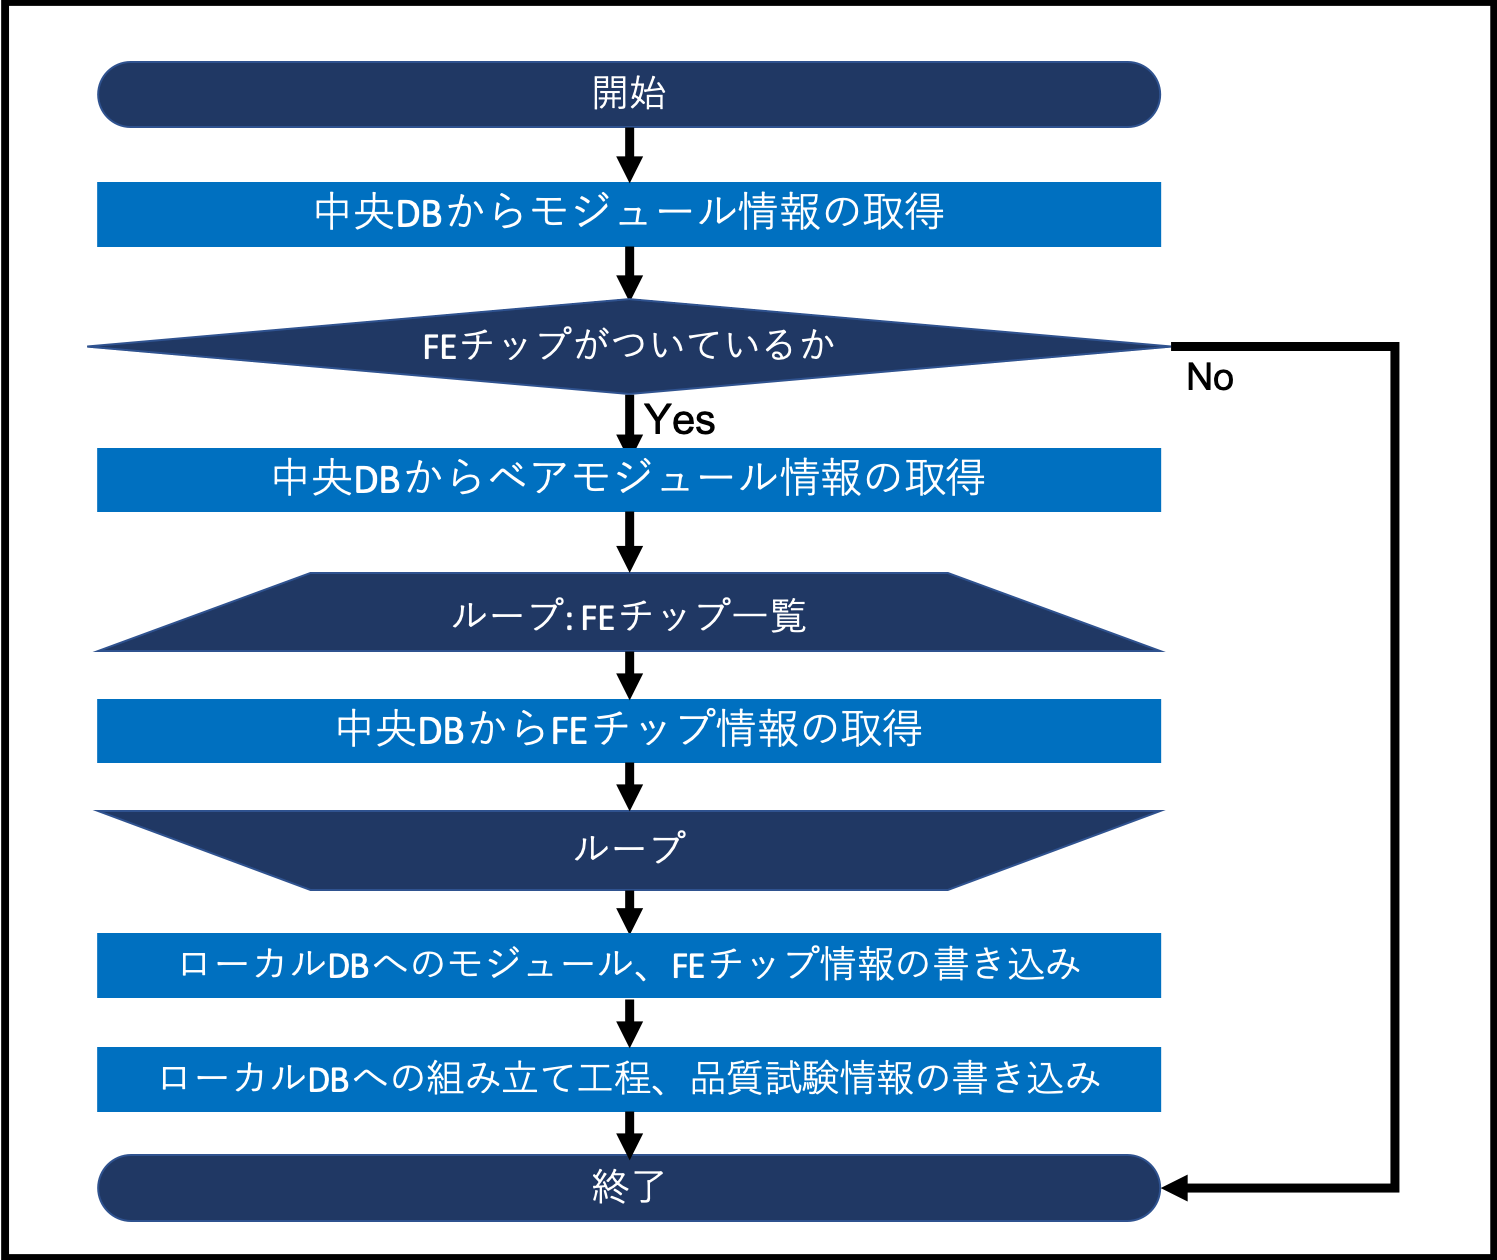
\includegraphics[width=11cm]{download_tool_flow_detail.png}
  \caption[ダウンロード処理に関する流れのイメージ図]{ダウンロード処理に関する流れのイメージ図}
  \label{download_algorithm}
  \end{center}
\end{figure}

\subsection{機能確認}
KEKで組み立てられた6台のモジュールを中央データベースに登録し、ダウンロードを行った。
登録したモジュールを表\ref{registered_kek_module}、ダウンロードをしてアプリケーションで確認した様子を図\ref{registered_kek_module_viewer}に示す。

\begin{table}[tbp]
\begin{center}
\caption[登録したKEKモジュール]{登録したKEKモジュール}
\label{registered_kek_module}
  \begin{tabular}{|ll|} \hline
    1 & 2 \\ \hline
    result 1 & result 2 \\ \hline 
  \end{tabular}
\end{center}
\end{table}

\begin{figure}[bpt]\centering

\includegraphics[width=1cm]{figure}
\caption[ダウンロードしたKEKモジュールがアプリケーションで確認できている様子]{ダウンロードしたKEKモジュールがアプリケーションで確認できている様子}
\label{registered_kek_module_viewer}
\end{figure}

\subsection{処理時間測定}
KEKモジュールをダウンロードした際の処理時間を測定した。
これについてまとめたものを表\ref{download_measurement}に示す。

\begin{table}[tbp]
\begin{center}
\caption[ダウンロード処理時間測定]{ダウンロード処理時間測定}
\label{download_measurement}
  \begin{tabular}{|ll|} \hline
    1 & 2 \\ \hline
    result 1 & result 2 \\ \hline 
  \end{tabular}
\end{center}
\end{table}

\subsection{生産時における見積もり}

\subsection{改善点}

\section{読み出し試験結果のアップロード機能確認と処理時間測定}
4章で述べたように、読み出し試験結果について中央データベースへアップロードするツールを開発した。
以下で詳細を述べる。
\subsection{アップロードする情報とその構造}
読み出し試験結果について、中央データベースにアップロードする情報を以下に記す。
\begin{itemize}
  \item 試験日時
  \item モジュール周りの環境温度
  \item ピクセル解析結果 
  \item 各試験結果データファイル
  \item 読み出し設定ファイル
  \item その他設定ファイル(DB、ユーザ、組み立て機関等)
\end{itemize}

中央データベースにおける読み出し試験の構造に関して、YARRを用いて行った読み出し結果は全てFEチップ毎に取得、保存される。
そのため、データベースの内部でもFEチップに読み出し試験結果を紐つける構造を設け、モジュールの結果では、各FEチップの結果ページのIDを持つ構造とした。イメージを図\ref{structure_for_electrical_tests}に示す。

\begin{figure}[bpt]\centering
  \begin{center}
  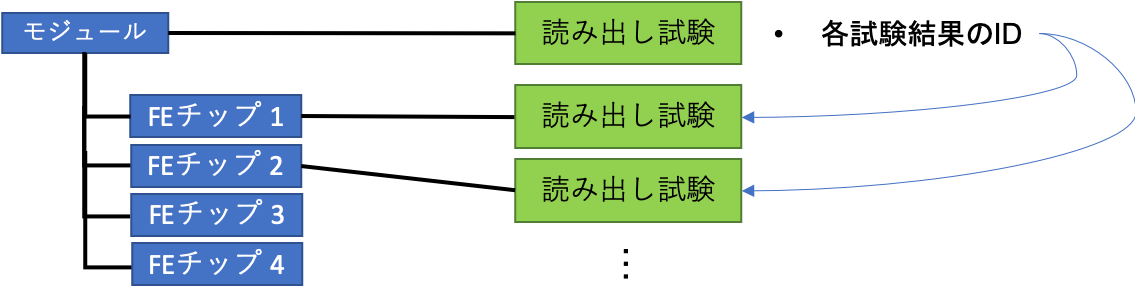
\includegraphics[width=13cm]{structure_for_electrical_tests.png}
  \caption[中央データベースにおける読み出し試験結果の構造]{中央データベースにおける読み出し試験結果の構造}
  \label{structure_for_electrical_tests}
  \end{center}
\end{figure}

また中央データベースにおいてモジュール、FEチップの試験結果が持つ情報を表\ref{electrical_parameters}にまとめる。
\begin{table}[tbp]
\begin{center}
\caption[ダウンロード処理時間測定]{ダウンロード処理時間測定}
\label{electrical_parameters}
  \begin{tabular}{|l|l|l|} \hline
    部品 & 試験情報、結果 & 添付ファイル \\ \hline\hline
    モジュール &  モジュール環境温度 & \\  
               &  FEチップにつく読み出し試験結果のID & \\  \hline
    FEチップ &  ピクセル解析結果 & 試験結果データファイル\\ 
             &                   & 読み出し設定ファイル\\
             &                   & その他設定ファイル\\ \hline 
  \end{tabular}
\end{center}
\end{table}

\subsection{処理の流れ}
アップロード機能における処理の流れのイメージを図\ref{upload_algorithm}に示す。
\begin{figure}[bpt]\centering
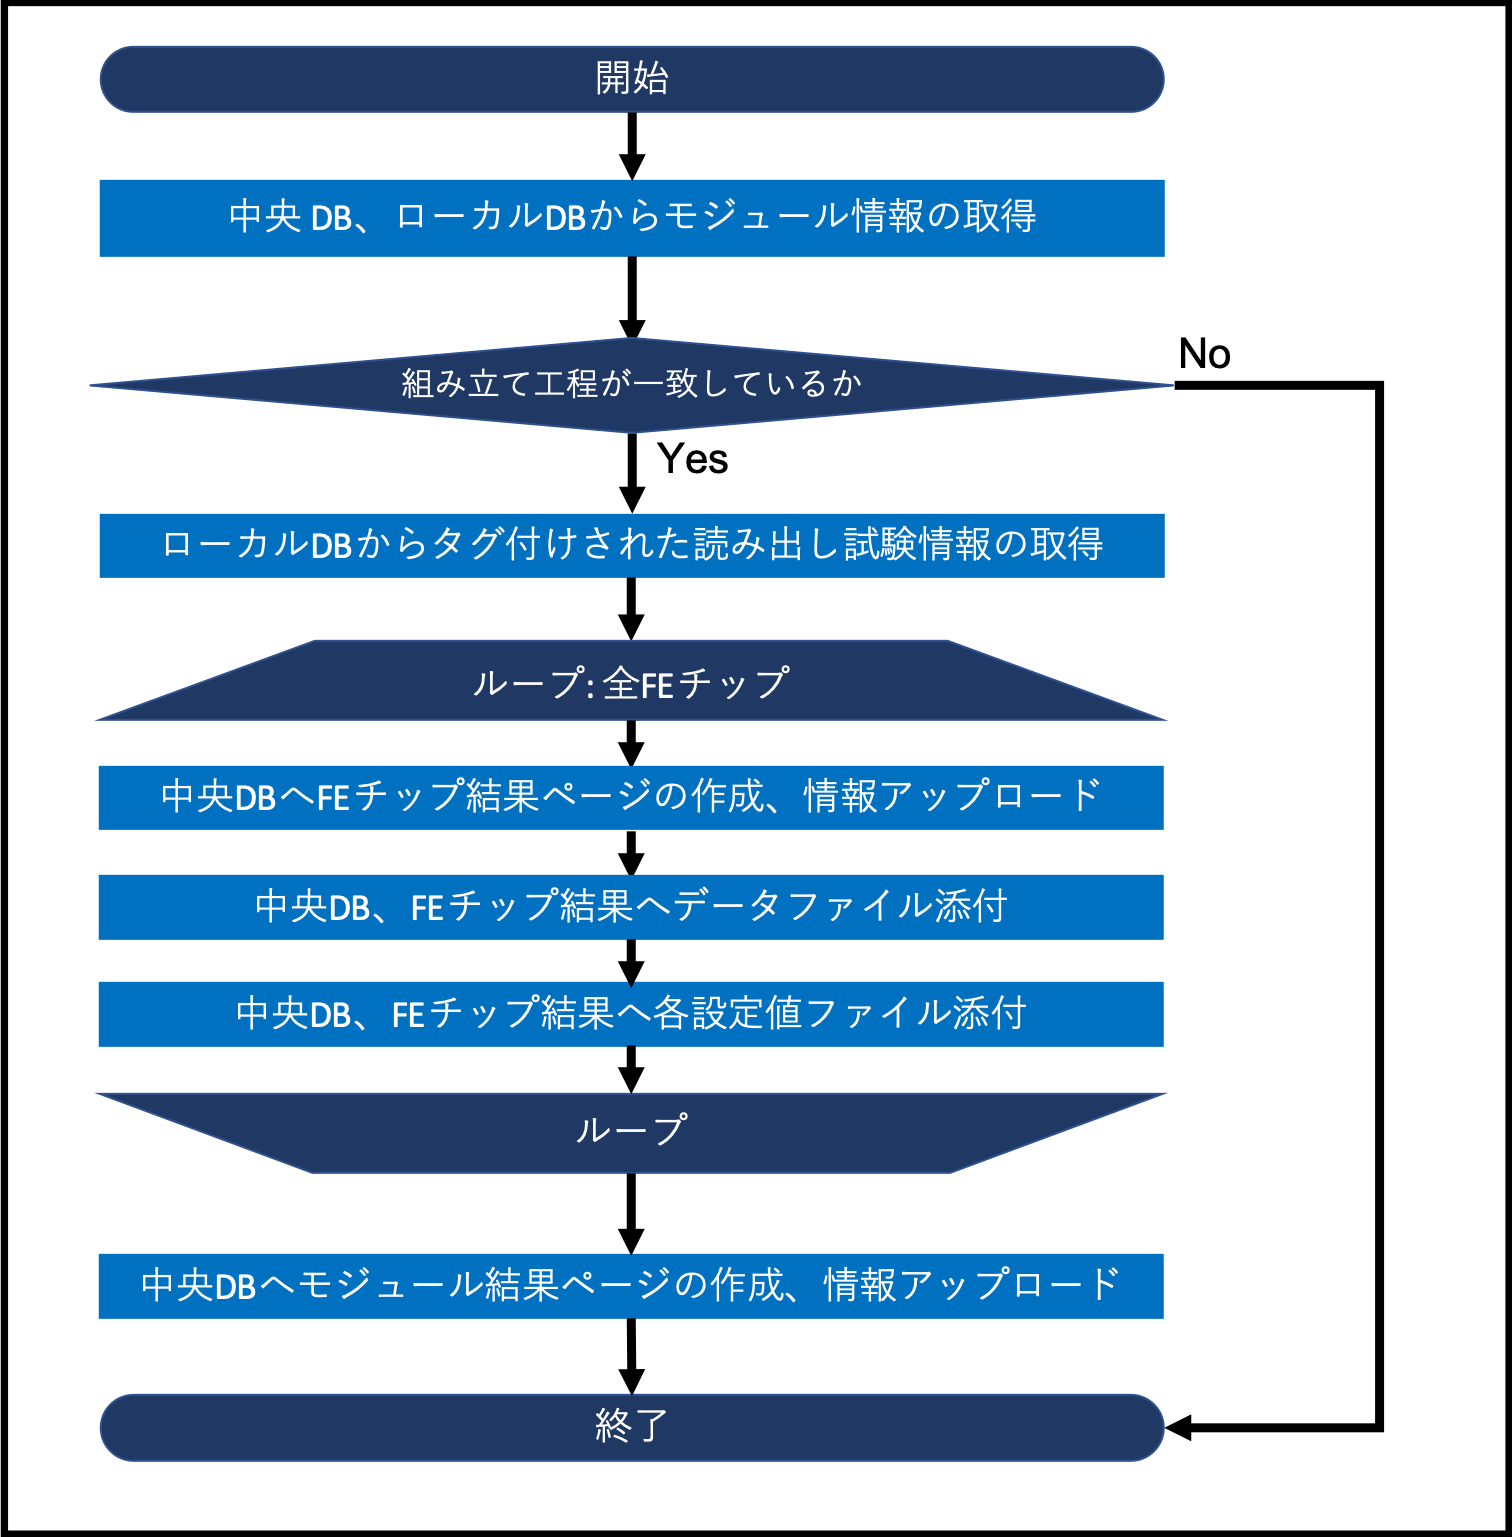
\includegraphics[width=10cm]{upload_algorithm}
\caption[アップロード処理に関する流れのイメージ図]{アップロード処理に関する流れのイメージ図}
\label{upload_algorithm}
\end{figure}

\subsection{機能確認と問題点}
上述した処理のツールを開発し、機能確認と処理時間測定を行った。
その際以下のような問題点があった。
\begin{itemize}
  \item 処理時間が長い。
  \item ファイルの容量制限により、データ容量が4MBを超えるファイルの添付に失敗した。
\end{itemize}

問題1の改善に向けて、アップロードにかかる時間を測定した。
KEKのサーバーを用いて、20回アップロード処理を行い、かかる時間を測定した。
その平均を測定値とした。

以下のようになった。
\bbb
  (1.3 \pm 0.0) \times 10^2 [{\rm sec}]
\eee

処理時間を改善するにあたって、処理時間詳細測定を行った。表\ref{upload_algorithm}より特に以下の詳細処理を抜粋し、それぞれにかかる時間を測定した。
\begin{enumerate}
  \item 中央データベース接続、認証。
  \item 中央データベース、ローカルデータベースからモジュール情報の取得。
  \item 中央データベースにFEチップ結果ページの作成。結果情報をアップロード。
  \item 2で作成した結果に対して、各データファイルを添付。
  \item 2で作成した結果に対して、各設定値ファイルを添付。
  \item 中央データベースにモジュールの結果ページの作成。結果情報をアップロード。
\end{enumerate}

測定条件は上記のものと同じとする。
結果を表\ref{upload_process_detail_result}に示す。
\begin{table}[tbp]
\begin{center}
\caption[アップロード処理詳細結果]{アップロード処理詳細結果}
\label{upload_process_detail_result}
  \begin{tabular}{|ll|} \hline
    処理 & 時間[sec] \\ \hline
    1 & $ 14 \pm 0 $ \\  
    2 & $ 0.88 \pm 0.14 $ \\  
    3 & $ 2.2 \pm  0.1 $ \\  
    4 & $ 68 \pm 3 $ \\  
    5 & $ 44 \pm 0 $ \\ \hline 
    6 & $ 1.8 \pm 0.1 $ \\  
  \end{tabular}
\end{center}
\end{table}

それぞれの処理が全体に占める割合をグラフにしたものを表\ref{upload_process_detail_gragh}に示す。
\begin{figure}[bpt]\centering
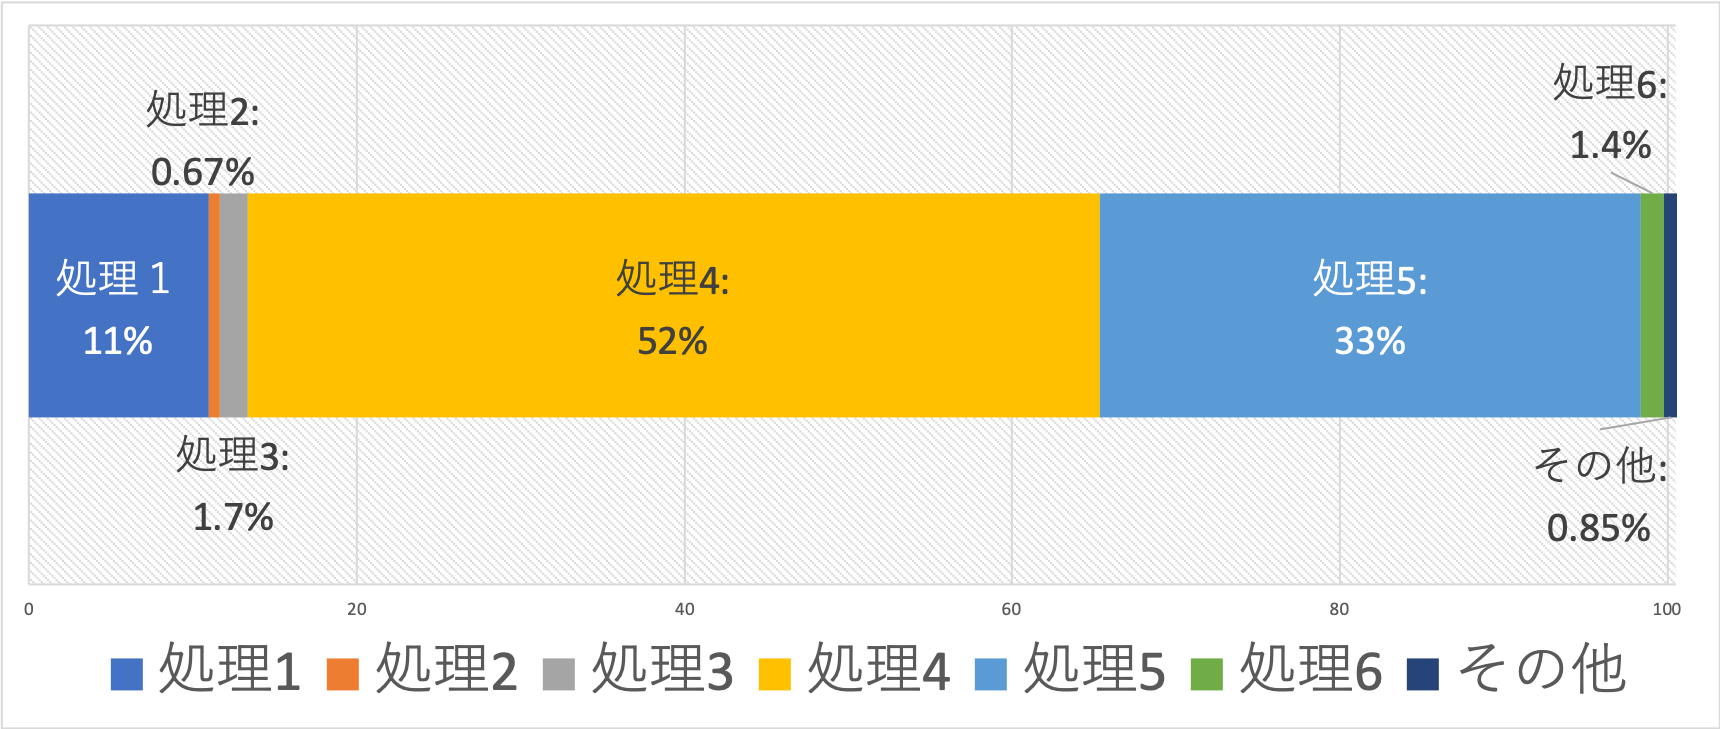
\includegraphics[width=10cm]{upload_process_detail_gragh}
\caption[アップロード時における各詳細処理が占める割合]{アップロード時における各詳細処理が占める割合}
\label{upload_process_detail_gragh}
\end{figure}
ファイル添付に多く時間がかかっていることがわかる。

各ファイル添付に対する処理時間の測定を行った。
添付する結果データファイル、設定ファイルの種類とデータ容量、添付処理実行結果、処理時間を表\ref{upload_status_to_pd}に示す。
問題点2にあげたように、4MBを超える容量のファイル添付は失敗していることがわかる。

\begin{longtable}{|llllll|}
  \caption[アップロード処理時のファイル添付実行結果]{アップロード処理時のファイル添付実行結果}
  \label{upload_status_to_pd}
  \endhead
  \hline
  読み出し項目 & ファイル名 & 実行結果 & 容量[KB] & 処理時間[sec] & 全体[sec]\\ 
  \hline
std$\_$digitalscan & EnMask.json & Ok & 1,300 & 3.3 $\pm$ 0.1 & 17$\pm$0 \\
 & OccupancyMap.json & Ok & 1.500 & 2.9 $\pm$ 0.2 & \\
 & L1Dist.json & Ok & 0.53 & 0.75 $\pm$ 0.12 & \\
 & ctrlCfg$\_$ctrlCfg.json & Ok & 0.46 & 0.61 $\pm$ 0.08 & \\
 & dbCfg$\_$dbCfg.json & Ok & 0.60 & 0.69 $\pm$ 0.16 & \\
 & siteCfg$\_$siteCfg.json & Ok & 0.033 & 0.61 $\pm$ 0.06 & \\
 & userCfg$\_$userCfg.json & Ok & 0.14 & 0.66 $\pm$ 0.09 & \\
 & scanCfg$\_$std$\_$digitalscan.json & Ok & 2.2 & 0.55 $\pm$ 0.06 & \\
 & beforeCfg$\_$chipCfg.json & { \bf Error} & 7,200 & 3.0 $\pm$ 0.2 & \\
 & afterCfg$\_$chipCfg.json & { \bf Error} & 7,200 & 4.0 $\pm$ 0.2 & \\
\hline
std$\_$analogscan & EnMask.json & Ok & 1,300 & 3.9 $\pm$ 0.1 & 17$\pm$0\\
 & OccupancyMap.json & Ok & 1.400 & 2.6 $\pm$ 0.1 & \\
 & L1Dist.json & Ok & 0.60 & 0.69 $\pm$ 0.16 & \\
 & ctrlCfg$\_$ctrlCfg.json & Ok & 0.46 & 0.54 $\pm$ 0.05 & \\
 & dbCfg$\_$dbCfg.json & Ok & 0.60 & 0.49 $\pm$ 0.04 & \\
 & siteCfg$\_$siteCfg.json & Ok & 0.033 & 0.48 $\pm$ 0.04 & \\
 & userCfg$\_$userCfg.json & Ok & 0.14 & 0.58 $\pm$ 0.08 & \\
 & scanCfg$\_$std$\_$analogscan.json & Ok & 2.1 & 0.45 $\pm$ 0.03 & \\
 & beforeCfg$\_$chipCfg.json & { \bf Error} & 7,200 & 2.9 $\pm$ 0.2 & \\
 & afterCfg$\_$chipCfg.json & { \bf Error} & 7,200 & 3.9 $\pm$ 0.3 & \\
\hline
std$\_$thresholdscan & Scurve-30-96.json & Ok & 0.98 & 1.3 $\pm$ 0.1 & 49$\pm$1\\
 & Scurve-110-96.json & Ok & 0.98 & 0.45 $\pm$ 0.03 & \\
 & Scurve-70-96.json & Ok & 0.98 & 0.47 $\pm$ 0.04 & \\
 & Scurve-150-96.json & Ok & 1.0 & 0.46 $\pm$ 0.04 & \\
 & Scurve-190-96.json & Ok & 1.0 & 0.64 $\pm$ 0.12 & \\
 & Scurve-230-96.json & Ok & 1.0 & 0.49 $\pm$ 0.03 & \\
 & Scurve-270-96.json & Ok & 1.0 & 0.47 $\pm$ 0.04 & \\
 & Scurve-310-96.json & Ok & 1.0 & 0.47 $\pm$ 0.04 & \\
 & Scurve-350-96.json & Ok & 1.0 & 0.49 $\pm$ 0.03 & \\
 & Scurve-390-96.json & Ok & 1.0 & 0.52 $\pm$ 0.06 & \\
 & Scurve-40-96.json & Ok & 1.0 & 0.46 $\pm$ 0.03 & \\
 & Scurve-80-96.json & Ok & 0.99 & 0.68 $\pm$ 0.13 & \\
 & Scurve-120-96.json & Ok & 1.0 & 0.54 $\pm$ 0.07 & \\
 & Scurve-160-96.json & Ok & 1.0 & 0.51 $\pm$ 0.05 & \\
 & Scurve-200-96.json & Ok & 1.0 & 0.49 $\pm$ 0.04 & \\
 & Scurve-240-96.json & Ok & 1.0 & 0.50 $\pm$ 0.05 & \\
 & Scurve-280-96.json & Ok & 1.0 & 0.48 $\pm$ 0.04 & \\
 & Scurve-320-96.json & Ok & 1.0 & 0.49 $\pm$ 0.05 & \\
 & Scurve-360-96.json & Ok & 1.0 & 0.49 $\pm$ 0.06 & \\
 & Scurve-400-96.json & Ok & 1.0 & 0.45 $\pm$ 0.05 & \\
 & Scurve-10-96.json & Ok & 1.0 & 0.42 $\pm$ 0.03 & \\
 & Scurve-50-96.json & Ok & 0.99 & 0.49 $\pm$ 0.05 & \\
 & Scurve-90-96.json & Ok & 0.99 & 0.46 $\pm$ 0.05 & \\
 & Scurve-130-96.json & Ok & 1.0 & 0.47 $\pm$ 0.05 & \\
 & Scurve-170-96.json & Ok & 1.0 & 0.52 $\pm$ 0.04 & \\
 & Scurve-210-96.json & Ok & 1.0 & 0.51 $\pm$ 0.04 & \\
 & Scurve-250-96.json & Ok & 1.0 & 0.58 $\pm$ 0.10 & \\
 & Scurve-290-96.json & Ok & 1.0 & 0.64 $\pm$ 0.13 & \\
 & Scurve-330-96.json & Ok & 1.0 & 0.64 $\pm$ 0.09 & \\
 & Scurve-370-96.json & Ok & 1.0 & 0.49 $\pm$ 0.06 & \\
 & Scurve-60-96.json & Ok & 0.99 & 0.51 $\pm$ 0.06 & \\
 & Scurve-100-96.json & Ok & 1.0 & 0.48 $\pm$ 0.05 & \\
 & Scurve-140-96.json & Ok & 1.0 & 0.48 $\pm$ 0.06 & \\
 & Scurve-180-96.json & Ok & 1.0 & 0.52 $\pm$ 0.06 & \\
 & Scurve-220-96.json & Ok & 1.0 & 0.54 $\pm$ 0.05 & \\
 & Scurve-260-96.json & Ok & 1.0 & 0.51 $\pm$ 0.05 & \\
 & Scurve-300-96.json & Ok & 1.0 & 0.66 $\pm$ 0.09 & \\
 & Scurve-340-96.json & Ok & 1.0 & 0.51 $\pm$ 0.06 & \\
 & Scurve-380-96.json & Ok & 1.0 & 0.55 $\pm$ 0.05 & \\
 & sCurve-0.json & Ok & 49 & 1.0 $\pm$ 0.1 & \\
 & ThresholdDist-0.json & Ok & 4.6 & 0.56 $\pm$ 0.06 & \\
 & ThresholdMap-0.json & Ok & 2,200 & 4.3 $\pm$ 0.1 & \\
 & NoiseDist-0.json & Ok & 2.3 & 0.42 $\pm$ 0.04 & \\
 & Chi2Map-0.json & Ok & 2,300 & 4.5 $\pm$ 0.1 & \\
 & StatusMap-0.json & Ok & 1,300 & 2.8 $\pm$ 0.1 & \\
 & StatusDist-0.json & Ok & 0.49 & 0.48 $\pm$ 0.04 & \\
 & NoiseMap-0.json & Ok & 2,200 & 4.0 $\pm$ 0.2 & \\
 & Chi2Dist-0.json & Ok & 1.1 & 0.50 $\pm$ 0.04 & \\
 & TimePerFitDist-0.json & Ok & 3.1 & 0.56 $\pm$ 0.12 & \\
 & ctrlCfg$\_$ctrlCfg.json & Ok & 0.46 & 0.49 $\pm$ 0.05 & \\
 & dbCfg$\_$dbCfg.json & Ok & 0.60 & 0.52 $\pm$ 0.06 & \\
 & siteCfg$\_$siteCfg.json & Ok & 0.033 & 0.54 $\pm$ 0.07 & \\
 & userCfg$\_$userCfg.json & Ok & 0.14 & 0.60 $\pm$ 0.07 & \\
 & scanCfg$\_$std$\_$thresholdscan.json & Ok & 2.2 & 0.46 $\pm$ 0.03 & \\
 & beforeCfg$\_$chipCfg.json & { \bf Error} & 7,200 & 3.2 $\pm$ 0.2 & \\
 & afterCfg$\_$chipCfg.json & { \bf Error} & 7,200 & 3.5 $\pm$ 0.1 & \\
\hline
std$\_$totscan & MeanTotMap-0.json & Ok & 1,900 & 4.8 $\pm$ 0.1 & 20$\pm$0\\
 & SigmaTotMap-0.json & Ok & 2,200 & 4.1 $\pm$ 0.2 & \\
 & MeanTotDist-0.json & Ok & 0.59 & 0.54 $\pm$ 0.07 & \\
 & SigmaTotDist-0.json & Ok & 1.8 & 0.47 $\pm$ 0.03 & \\
 & L1Dist.json & Ok & 0.59 & 0.60 $\pm$ 0.08 & \\
 & ctrlCfg$\_$ctrlCfg.json & Ok & 0.46 & 0.47 $\pm$ 0.03 & \\
 & dbCfg$\_$dbCfg.json & Ok & 0.60 & 0.67 $\pm$ 0.24 & \\
 & siteCfg$\_$siteCfg.json & Ok & 0.033 & 0.59 $\pm$ 0.10 & \\
 & userCfg$\_$userCfg.json & Ok & 0.14 & 0.56 $\pm$ 0.05 & \\
 & scanCfg$\_$std$\_$totscan.json & Ok & 2.0 & 0.59 $\pm$ 0.10 & \\
 & beforeCfg$\_$chipCfg.json & { \bf Error} & 7,200 & 3.0 $\pm$ 0.1 & \\
 & afterCfg$\_$chipCfg.json & { \bf Error} & 7,200 & 3.9 $\pm$ 0.3 & \\
\hline
std$\_$noisescan & Occupancy.json & Ok & 1,300 & 4.0 $\pm$ 0.1 & 18$\pm$0\\
 & NoiseOccupancy.json & Ok & 1,300 & 2.5 $\pm$ 0.1 & \\
 & NoiseMask.json & Ok & 1,300 & 2.4 $\pm$ 0.1 & \\
 & ctrlCfg$\_$ctrlCfg.json & Ok & 0.46 & 0.57 $\pm$ 0.08 & \\
 & dbCfg$\_$dbCfg.json & Ok & 0.60 & 0.55 $\pm$ 0.06 & \\
 & siteCfg$\_$siteCfg.json & Ok & 0.033 & 0.53 $\pm$ 0.04 & \\
 & userCfg$\_$userCfg.json & Ok & 0.14 & 0.61 $\pm$ 0.07 & \\
 & scanCfg$\_$std$\_$noisescan.json & Ok & 1.4 & 0.53 $\pm$ 0.05 & \\
 & beforeCfg$\_$chipCfg.json & { \bf Error} & 7,200 & 2.8 $\pm$ 0.2 & \\
 & afterCfg$\_$chipCfg.json & { \bf Error} & 7,200 & 3.5 $\pm$ 0.1 & \\
\hline
\end{longtable}

\subsubsection{生産時における見積もり}
Quadモジュールにおいて、1つのモジュールに対する生産時のアップロード処理合計時間の見積もりを以下で行った。
上述した測定はSCCであるため、FEチップに対する処理は1回である。Quadの場合は4回分であることを考慮すると、モジュール1つに対して以下のように見積もることができる。
\bbb
hogehoge
\eee

\subsection{改善策}

容量を減らし、APIの使用回数を減らす。

合計処理時間は以下のようになった。??$\%$の削減に成功した。


\begin{longtable}{|llllll|}
  \caption[アップロード処理時のzipファイル添付実行結果]{アップロード処理時のzipファイル添付実行結果}
  \label{upload_status_to_pd_zip}
  \endhead
  \hline
  読み出し項目 & ファイル名 & 添付処理実行結果 & データ容量[KB] & 処理時間[sec] & 削減率[$\%$] \\ 
  \hline
  std$\_$digitalscan & datafile.zip & Ok & 1,300 & & \\
                     & configfile.zip & Ok & 7,200 & &\\
  \hline
\end{longtable}

\subsubsection{生産時における見積もり}
十分に運用可能であると考えられる。

